\part{General concepts \protect\\
      Version control}
      
\frame{\partpage}

    
    
\section{Introduction}
%---------------------



    \subsection{Reproducibility}
    %---------------------------



\begin{frame}{A common problem}

    \begin{center}
    
        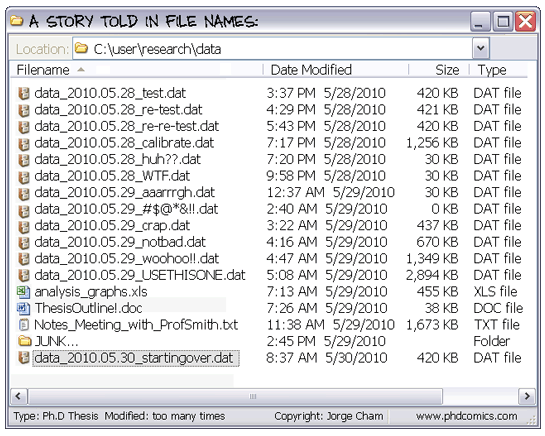
\includegraphics[width=0.6\textwidth]{../images/phd052810s.png}
    
        \pause
    
        Not only with data, but also with scripts

    \end{center}
    
        
\end{frame}


\begin{frame}{Reproducibility ?}
    
    \begin{itemize}
        
        \item Research should be reproducible by others.
        
        \pause
        
        \item This refers to the experiments generating the data, but also 
          to the analysis of the data.
          
        \pause
        
        \item The first researcher who will need to reproduce the results is
          you.
        
    \end{itemize}
    
\end{frame}



\begin{frame}{Reproducibility of analysis}
    
    \begin{itemize}
        
        \item Lab books make lab work traceable. Analysis should also be 
          traceable.
        
        \pause
        
        \item Analysis steps must be logged, and reverting to any previous step
          must be possible.
        
        \pause
        
        \item This ensures that we always exactly know how a result was 
          generated. 
        
    \end{itemize}
    
\end{frame}



\begin{frame}{Version control}
    
    \begin{itemize}
        
        \item Version control is a tool to keep track of file changes.
        
        \pause
        
        \item However, version control softwares offer more than simply 
          recording successive versions of a file.
          
        \pause
        
        \item Version controlled projects can be splitted, merged and shared
          with collaborators.
        
    \end{itemize}

\end{frame}



\begin{frame}{Version control flow}
    
    \tikzstyle{version} = [circle, fill = blue!15]
    
    \tikzstyle{branch} = [circle, fill = green!30]
    
    \tikzstyle{merge} = [circle, fill = blue!30]
    
    \tikzstyle{bad_version} = [circle, fill = red!50]
    
    \begin{figure}
        
        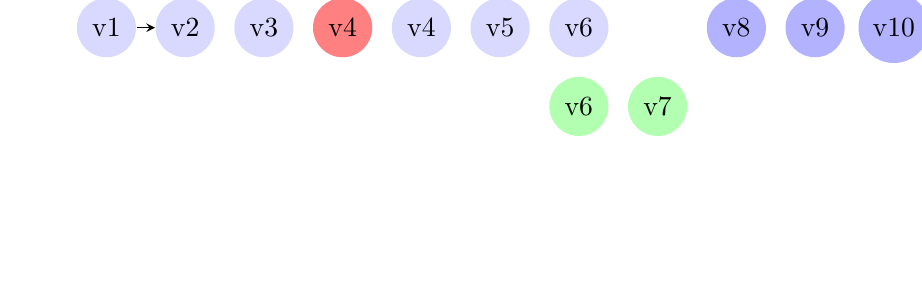
\begin{tikzpicture}[>=stealth]
                    
            \path[use as bounding box] (-1, 0) rectangle (10, -3);
            
            \path[->]<1-> node[version](v1){v1};
            
            \path[->]<2-> node[version, right of = v1](v2){v2}
            
                          (v1) edge node {} (v2);
            
            \path[->]<3-> node[version, right of = v2](v3){v3};
            
            \path[->]<4-> node[version, right of = v3](v4){v4};
            
            \path[->]<5-> node[bad_version, right of = v3](v4bad){v4};
            
            \path[->]<6-> node[version, right of = v4](v4ok){v4};
            
            \path[->]<7-> node[version, right of = v4ok](v5){v5};
            
            \path[->]<8-> node[right of = v5](empty1){};
            
            \path[->]<8-> node[branch, below of = empty1](v6b){v6};
            
            \path[->]<9-> node[branch, right of = v6b](v7b){v7};
            
            \path[->]<10-> node[version, right of = v5](v6a){v6};
            
            \path[->]<11-> node[right of = v6a](empty2){};
            
            \path[->]<11-> node[merge, right of = empty2](v8){v8};
            
            \path[->]<12-> node[merge, right of = v8](v9){v9}
            
                           (v1) -- +(0, 1) -| node {} (v9);
            
            \path[->]<13-> node[merge, right of = v9](v10){v10};
            
        \end{tikzpicture}
        
        
    \end{figure}
    
\end{frame}




\begin{frame}{Example of project structure}
    
    blabla
    
\end{frame}


\begin{frame}{Keeping track}
    
    What reproducibiity means
    
\end{frame}




    \subsection{Tools needed}
    %------------------------





\section{Version control}
%------------------------



    \subsection{Interest of version control}
    %---------------------------------------
    
    
    
    \subsection{Multiple users, single user}
    %---------------------------------------
    
    
    
    \subsection{Version control depository}
    %--------------------------------------


\section{Version control with R}
%-------------------------------

\subsection{Setting up the project}

\subsection{example}



\begin{frame}
    
    useful links and references
    
\end{frame}

data : from http://ocean.ices.dk/HydChem/HydChem.aspx?plot=yes


